\chapter{Preparazione DNA plasmidico tramite lisi alcalina}

\vspace{0.6cm}


\section{Sommario}

\subsection{Scopo}

L'obiettivo di questa esperienza è quello di effettuare una miniprep, cioè una Minipreparazione di DNA plasmidico.
Dovremmo perciò andare tramite una lisi a rompere la membrana cellulare per estrarne il DNA plasmidico, per poterlo
utilizzare nelle procedure di trasfezione.

\subsection{Cenni teorici}

La miniprep è una tecnica di laboratorio utilizzata per prelevare, in piccole quantità,
del DNA plasmidico dai batteri che lo contengono.

Innanzitutto andiamo a vedere nel dettaglio cos'è il DNA plasmidico.
I plasmidi sono piccoli filamenti circolari di DNA superavvolto a doppia elica,
presenti nel citoplasma di tutti i batteri;
sono delle molecole estracromosomiali auto replicanti.
In natura i plasmidi assumono strutture diverse, grandezze diverse, numero di copie diverse e modi
di replicazione differenti in base al batterio che li contiene.
Questi plasmidi hanno l'abilità di propagarsi in batteri differenti, trasferirsi tra specie
batteriche e forse la più importante sono i tratti genetici che trasportano.

\begin{figure}[H]

	\centering
	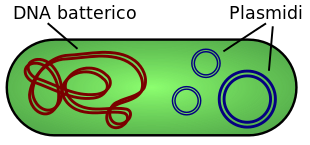
\includegraphics[width=0.6\textwidth]{./immagini/plasmide.png}
	\caption{illustrazione cellula batterica con DNA batterico (rosso) e DNA plasmidico (blu).}
	\label{plasmide}

\end{figure}

L'uso dei plasmidi è molto ingegnoso, in quanto permette di replicare il materiale genico all'interno dei batteri
oppure di trasferire determinati geni in altri organismi.


\subsection{Materiali utilizzati}

\begin{itemize}
	\item Guanti in lattice
	\item Micropipette (\SI{100}{\micro\liter}-\SI{1000}{\micro\liter} e \SI{2}{\micro\liter}-\SI{200}{\micro\liter}  )
	\item Eppendorf (2ml)
\end{itemize}


\subsection{Soluzioni utilizzate}

\begin{itemize}

	\item Soluzione I:
  \begin{enumerate}
    \item 50 mM glucosio
    \item 25 mM Tris-HCL (pH 8.0)
    \item 10 mM EDTA (pH 8.0)
  \end{enumerate}
	\item Soluzione II:
  \begin{enumerate}
    \item 0.2 NaOH
    \item 1 \% SDS
  \end{enumerate}
	\item Soluzione III:
  \begin{enumerate}
    \item 5M potassio acetato 60 mL
    \item acido acetico glaciale 11.5 mL
    \item acqua distillata 28.5 mL
  \end{enumerate}

\end{itemize}

\vspace{0.5cm}

\textbf{NOTE:}
\begin{itemize}
  \item La soluzione I è necessaria per risospendere le cellule e portarle in condizioni
	adatte per la successiva lisi;
  \item La soluzione II provoca la lisi alcalina delle cellule grazie a NaOH che denatura
	il DNA e l’SDS che è un detergente e denatura le proteine.
\end{itemize}


\section{Procedimento}

\subsection{Miniprep:}

\begin{enumerate}
  \item Prelevare 1.5ml di coltura batterica fresca, in quanto l’utilizzo di colture vecchie potrebbe
	influenzare negativamente la corretta purificazione del DNA, a causa dell’accumulo di metaboliti secondari.
	Non è rilevante la quantità di coltura batterica che si preleva ma \`e meglio prenderne abbastanza da riempire
	l’eppendorf, in modo da massimizzare la quantità di DNA. Non è indispensabile l’utilizzo di una cappa sterile:
	l’eventuale presenza di DNasi esogene viene contrastata con l’utilizzo, nelle fasi successive, di EDTA.
  \item Centrifugare per 30’’ a 12.000rpm (non serve che la centrifuga sia a 4°C, si pu\`o centrifugare direttamente
	a temperatura ambiente) per consentire la formazione di un pellet più o meno
	compatto (quelli riportati sono valori di centrifugazione indicativi: se il pellet è instabile procedere
	con un’ulteriore centrifugazione). Finita la centrifuga eliminare il surnatante versando il contenuto del tubo picchiettando
	leggermente con il tappo aperto, in modo da allontanare il più possibile eventuali gocce dal terreno,
	per non modificare le concentrazioni delle tre soluzioni che verranno usate in seguito.

  \item Risospendere il pellet batterico in 100 μl di Soluzione I. Per la risospensione si può utilizzare il vortex o
	il puntale di una pipetta, in quanto le cellule sono ancora integre ed il DNA è protetto.

  \item Aggiungere 200 μl di Soluzione II e mescolare. Essendo una soluzione alcalina provoca la lisi delle cellule,
	la denaturazione e la  precipitazione delle molecole di DNA genomico e plasmidico.
	Le molecole di DNA a causa della lisi diventano estremamente fragili, per questo si deve mescolare
	adeguatamente evitando per\`o azioni troppo energiche (vortex) per non rompere il DNA stesso.
	Come risultato si ottiene un lisato cellulare viscoso e biancastro.

  \item Aggiungere 150 μl di soluzione III entro 2-3 minuti dall’aggiunta della Soluzione II e
	mescolare capovolgendo il tubo due o tre volte in maniera delicata (non vortexare).
	Aggiungendo la soluzione III si riporta il lisato cellulare a pH che permette la rinaturazione del DNA plasmidico.
	La tempistica che precede l’aggiunta della soluzione III è fondamentale per la separazione del DNA plasmidico dal genomico:
	il DNA plasmidico, proprio perché superavvolto e di piccole dimensioni, se mantenuto in condizioni di lisi per un tempo non
	superiore ai 3-4 minuti riesce a rinaturare, mentre il DNA genomico e le proteine rimangono intrappolate irreversibilmente nel
	complesso formato da potassio e SDS. Nel caso la soluzione II venisse lasciata agire per periodi più lunghi,
	il DNA plasmidico sarebbe comunque in grado di rinaturare ma assumerebbe una conformazione tale da risultare inattaccabile
	dagli enzimi di restrizione.

  \item Centrifugare a massima velocità per 5 minuti per permettere la sedimentazione dei residui cellulari e recuperare
	il surnatante in un nuovo tubo. E’ consigliato prelevare una quantità non superiore a 550μl.
	Questo perché verrà aggiunto un volume doppio di etanolo nelle fasi successive.

  \item OPZIONALE : Trattamento con fenolo-cloroformio per eliminare le proteine rimanenti. Questo trattamento verrà
	spiegato singolarmente più avanti.

  \item Precipitare il DNA con due vol. di etanolo (100\% v/v) oppure con 0.6 vol. di isopropanolo. L'etanolo è aggiunto
	al 100\% per ottenere una soluzione finale al 70\%. Per esempio: a 100 μl di DNA si aggiungono 200 μl di etanolo
	assoluto oppure 60 μl di isopropanolo. In questa fase è necessario capovolgere il tubo delicatamente, infatti il DNA
	deve venire a contatto con l’alcol per precipitare.

  \item Centrifugare a 12.000g per 5 minuti. In caso il DNA sia sporco è possibile che sia presente del il pellet bianco sul fondo del tubo.
	Invece in presenza di una grande quantità di polisaccaridi il pellet è mucillaginoso.

  \item Rimuovere il supernatante e lavare con etanolo 70\% v/v, che permette di eliminare i sali rimasti.
	Per eliminare l’etanolo effettuare un breve passaggio in centrifuga (30” a massima velocità) per far scendere eventuali
	goccioline sul fondo del tubo e quindi aspirarle con una micropipetta, oppure capovolgere la provetta e scuoterla
	leggermente sulla carta. Versare nel tubo circa 500 μl di EtOH 70\%.

  \item Rimuovere completamente l’etanolo aspirandolo con una micropipetta senza rompere il pellet e lasciarlo asciugare
	all’aria per 10 minuti. L’asciugatura può essere velocizzata ponendo la provetta in un luogo ben aerato,
	come ad esempio una cappa a flusso laminare.
	\`E importante che il pellet sia completamente asciutto perché la presenza di tracce di etanolo determina una scarsa
	risospensione del DNA e, soprattutto, ne provoca la fuoriuscita dal pozzetto quando si effettua il caricamento su gel di
	agarosio per un’elettroforesi.

  \item Risospendere il DNA plasmidico in 50 μl di TE pH 8.0 che permette la risospensione evitando la degradazione.
	Infatti, il TE è composto da EDTA che garantisce protezione dalle DNAsi.

  \item Conservare a 4°C. Se si opta per una risospensione in acqua si deve conservare a –20°C.

\end{enumerate}

\subsection{Trattamento con Fenolo-cloroformio}

Il fenolo cloroformio è una soluzione sinergica altamente deproteinizzante che serve per eliminare i possibili
contaminanti del DNA (esempio: elimina proteine in sospensione in eccesso) per evitare che interferiscano con i
successivi trattamenti, specialmente nel caso in cui si lavori con enzimi di restrizione.
Questo trattamento può essere fatto anche su DNA genomico o comunque su DNA plasmidico già risospeso in TE.
Il passaggio in fenolo-cloroformio deve sempre esser seguito da precipitazione in etanolo assoluto (o isopropanolo)
e successiva risolubilizzazione in TE.

\begin{enumerate}
  \item Aggiungere alla soluzione contenente il DNA 1 vol. di fenolo:cloroformio:isoamilico (25:24:1)
	La presenza dell’isoamilico serve per semisaturare il cloroformio che altrimenti puro avrebbe la
	tendenza a disidratare il campione.

  \item Miscelare le due fasi (non vortexare) fintanto che il campione non si presenta lattiginoso.

  \item Centrifugare almeno 3 minuti in modo che si formino due fasi distinte:
	Una fase inferiore di fenolo-cloroformio e una superiore con il DNA in soluzione.
	L’interfaccia bianca è data dalle proteine denaturate.

  \item Recuperare la fase superiore, contenente il DNA, facendo attenzione a non
	prelevare anche la fase inferiore. Tenere la punta della pipetta appena sotto la superficie
	dello strato superiore (Fig.1). Ad un certo punto si forma una bolla di soluzione contenente il DNA.
	E’ consigliato tenere inclinato il tubo in modo da prevedere dove si formerà la bolla (Fig.2) contente il DNA in modo
	tale da prelevarne la maggior quantità possibile. Bisogna assolutamente evitare di trasportare il fenolo-cloroformio,
	perché questo andrebbe a degradare gli enzimi utilizzati in seguito.

  \item Precipitare il DNA con etanolo o isopropanolo. Se inizialmente il DNA era in TE, è necessario aggiungere 1/10 vol.
	NaOAc 3M pH 4.8 prima di aggiungere i 2 vol. di etanolo assoluto oppure gli 0.6 vol. isopropanolo.
	Qualora questo trattamento venga condotto durante la Miniprep (punto 5), la presenza massiccia di sali forniti con
	la Sol. III  rende inutile (se non dannosa) l’aggiunta di 1/10 vol. NaOAc 3M pH 4.8 prima dell’alcool.
	In questo caso la precipitazione deve essere condotta come da punto 6 del protocollo Miniprep.


\end{enumerate}

\section{Risultati e Conclusioni}

Come conclusione di questa esperienza, possiamo dire di aver capito come si possono estrarre dei frammenti di DNA (plasmidi)
dalle cellule batteriche di E.coli tramite questa lunga procedura, mentre nella prossima relazione spiegheremo per cosa
questi plasmidi verranno usati.
